\Chapter{MAGNIS (MAGnetized Negative Ion Source)}
\chaptermark{Modèles plasmas froids magnétisés}
Dans ce chapitre, nous proposons un nouveau modèle fluide pour décrire le
transport magnétisé dans les plasmas froids. Nous discutons tout d'abord de
l'approche standard de modélisation des plasmas froids, des problématiques qui
lui sont propres ainsi que des difficultés rencontrées lors du développement du
modèle basé sur les vitesses de dérive. La suite concerne l'élaboration du
nouveau modèle, nous le dérivons en expliquant les différents termes essentiels
à description du transport dans les plasmas froids puis nous détaillons le
schéma numérique original utilisé pour résoudre le modèle.
\section{Problématique}
La plupart des modèles fluides décrivant les phénomènes de transport magnétisés
dans les plasmas froids sont basés sur les équations de dérive-diffusion
(chapitre \ref{derivediffusion}). Cependant, au delà d'une certaine intensité de
champ magnétique, l'anisotropie du transport rend la résolution numérique de ces
équations complexe voire impossible\footnote{Le problème est alors généralement
adressé à travers le développement de modèles cinétiques numériquement très
coûteux, et nécessitant à priori la résolution d'échelles de l'ordre de la
longueur de Debye et de la fréquence plasma.}.
Celles-ci sont en fait peu adaptées au transport fortement
magnétisé~\citep{Golant}.


Un indice nous est donné en considérant la description du transport transverse
par les vitesses de dérive (cf.
introduction) où l'équilibre des courants fait intervenir la divergence de la
dérive de polarisation. Cette dérive, essentielle dans la dynamique du transport
transverse, est absente du modèle qui néglige totalement l'inertie des
particules. Le modèle de dérive-diffusion cherche une solution stationnaire à un
problème intrinsèquement non-stationnaire.

D'un autre côté,

\section{Description du modèle}
Le plasma est constitué d'électrons et d'une ou plusieurs espèces d'ions de
charge $q_s$ et de masse $m_s$. On considère un plasma de taille $L$, confiné et
en interaction avec des parois à travers une gaine large de quelques longueurs
de Debye. La longueur $L$ est prise suffisement grande $L\gg\lambda_D$ pour
supposer le plasma quasi-neutre. Le champ magnétique $\mathbf{B}$ imposé est de
plus stationnaire, de sorte que le champ électrique dérive directement d'un
potentiel électrostatique $\mathbf{E}=-\nabla \Phi$. Le transport est décrit
dans le plan perpendiculaire au champ magnétique et tient compte des pertes à la
paroi dans la direction parallèle en les intégrant le long des lignes de champ.

\subsection{Equations de conservation}
Comme discuté en introduction, nous retenons tous les termes de l'équation du
moment :
\begin{equation}
\partial_t \mathbf{u}_s + \mathbf{u}_s\cdot\nabla\mathbf{u}_s+
\nu_s\mathbf{u}_s+\omega_s\mathbf{b}\times\mathbf{u}_s=
-\frac{q_s}{m_s}\left(\nabla \Phi+\frac{\nabla p_s}{q_sn_s}\right)
\end{equation}

où $n_s$ est la densité de l'espèce considérée, $\mathbf{u}_s$ sa vitesse
fluide, $p_s$ la pression, $\Phi$ le potentiel électrostatique,
$\omega_s=q_sB/m_s$ la fréquence cyclotronique et $\nu_s$ la fréquence de collision effective.
Le transfert de quantité de mouvement dû aux collisions contient la perte liée à
l'ionization $\nu_s=\nu_{s}^{iz}+\nu_{s}^{sn}+\nu_{s}^{ie}$ où $\nu_{s}^{sn}$ et
$\nu_{s}^{ei}$ sont respectivement les fréquences de collisions particules
chargées - neutres et de collisions Coulombienne.

L'évolution de chaque espèce est décrite par une équation de continuité :
\begin{equation}
\label{3-continuite}
\partial_t n_s + \nabla\cdot\left(n_s\mathbf{u}_s\right)=S_s(T_e)
\end{equation}

avec $S_s$ un terme d'ionisation, fortement dépendant de la
température électronique $T_e$. En considérant l'hypothèse de quasi-neutralité, la somme des
équations de continuité conduit à l'équation de conservation du courant :
\begin{equation}
\label{eqCourant}
\nabla\cdot(\sum_ien_i\mathbf{u}_i-en_e\mathbf{u}_e)=0
\end{equation}

où l'indice i dénote éventuellement différentes espèces d'ions. Eq.
\ref{eqCourant} couple les différentes espèces en contrôlant l'évolution du potentiel électrostatique $U$.

L'équation de conservation de l'énergie est obtenue classiquement en substituant
l'équation de continuité afin d'éliminer le terme convectif :
\begin{equation}\begin{split}
\label{3-energie}
\frac{3}{2}n_e\partial_tT_e + \nabla\cdot(\mathbf{Q}) +
(\frac{5}{2}S_e-\partial_tn_e)T_e \\=n_e\mathbf{u}_e\cdot(\nabla
\Phi-\frac{5}{2}\nabla T_e)+n_e\left(P_{ext}-\Pi\right)
\end{split}
\end{equation}

où $T_e$ est la température électronique exprimée en eV, $S_e$ est le
terme source d'électrons lié à l'ionisation, $P_\text{ext}$ la puissance
extérieure déposée dans le plasma et $\Pi$ le terme de perte d'énergie dû aux collisions. La fermeture du modèle se fait alors sur le flux de chaleur
$\mathbf{Q}$~\citep{Golant} :
\begin{equation}
\partial_t \mathbf{Q} + \nu_e\mathbf{Q}+\omega_e\mathbf{Q}\times\mathbf{b} =
-\frac{5}{2}\frac{e^2}{m_e}n_eT_e\nabla T_e
\end{equation}

Le flux de chaleur est magnétisé de la même façon que le flux de matière et
dépend principalement du gradient de température. Dans les sources magnétisées,
où la longueur de gradient thermique est de l'ordre de grandeur de la largueur
du filtre magnétique, le flux de chaleur influence fortement le transport
transverse. Il doit donc nécessairement être pris en compte et décrit là encore
avec le minimum d'approximations.

\subsection{Conditions aux limites}
Le modèle est complété par la définition de conditions aux limites
portant sur les flux et intégrant le maximum de considérations physiques. Dans
le cas d'une paroi conductrice, un modèle classique de gaine non-collisionnelle
est utilisé. Les flux ioniques et le flux électronique sont définis en
l'entrée de gaine par :
\begin{align}
&\Gamma_i=\boldsymbol{\Gamma}_i\cdot\mathbf{n}=n.\max\left(c_s,\mathbf{u_i}\cdot\mathbf{n}\right)
\\
&\Gamma_e=\boldsymbol{\Gamma}_e\cdot\mathbf{n}=n\frac{1}{4}v_{th}=nc_s\exp(\Lambda-\Delta
\Phi/T_e)
\end{align}

avec $\mathbf{n}$ le vecteur normal à la paroi,
et $c_s=(eT_e/m_i)^{\text{\textonehalf}}$ la vitesse acoustique ionique.
La différence de potentiel entre le plasma et la
paroi se réécrit pour un courant nul:
\begin{equation}
	\mathbf{j}\cdot\mathbf{n}=0\Leftrightarrow \Delta \Phi=\Phi-\Phi_w =
T_e(\Lambda-ln\sum_i\Gamma_i/nc_s)
\end{equation} 

où le potentiel flottant $\Lambda$ est défini pour un plasma
n'étant composé que d'une espèce :
\begin{equation}
	\Lambda=ln\left(\frac{eT_e}{2\pi
	m_e\mathbf{u}_i^2}\right)^{\text{\textonehalf}} \le 
	ln\left(\frac{m_i}{2\pi m_e}\right)^{\text{\textonehalf}}
\end{equation}

Les ions sont perdus au minimum avec la vitesse acoustique, mais
éventuellement avec une vitesse supersonique. La condition limite pour le
courant est par conséquence définie par :
\begin{equation}
\boldsymbol{\Gamma}_\rho\cdot\mathbf{n}=\mathbf{j}\cdot\mathbf{n}=e\sum_i{\Gamma}_i-e{\Gamma}_e
\end{equation}

Si la paroi est isolante, la surface se polarise pour assurer la nullité du
courant sortant :
\begin{equation}\begin{split}
\boldsymbol{\Gamma}_\rho\cdot\mathbf{n}=0\Leftrightarrow
\Phi_w=\Phi-T_e(\Lambda-ln\sum_i\Gamma_i/nc_s)
\end{split}\end{equation}

L'énergie perdue par les électrons en entrée de gaine s'obtient en
additionnant l'énergie moyenne perdue à la paroi (intégrée sur une distribution
semi-maxwellienne) et l'énergie transférée aux ions dans la chute de potentiel :
\begin{equation}
	\varepsilon_w=2T_e+\Delta \Phi
\end{equation}
 
 On peut alors relier cette perte totale aux flux sortants de l'équation
 d'énergie Eq.\ref{3-energie}, correspondant au flux d'énergie porté par les
 particule et au flux de chaleur :
\begin{equation}
\boldsymbol{\Gamma}_\varepsilon=\frac{5}{2}\boldsymbol{\Gamma}_eT_e\cdot\mathbf{n}+\mathbf{Q}\cdot\mathbf{n}=
\boldsymbol{\Gamma}_e\left(2T_e+\Delta\Phi\right)\cdot\mathbf{n}
\end{equation}

En regroupant les termes portant sur le flux d'électron, on peut exprimer la
condition limite pour le flux de chaleur :
\begin{equation}
\mathbf{Q}\cdot\mathbf{n}=\Gamma_e\left(\Delta\Phi-\frac{1}{2}T_e\right)
\end{equation}

Ces conditions aux limites sont justifiées dans des plasmas non-magnétisés et à
l'extrémité de lignes de champ interceptant perpendiculairement la paroi dans
des plasmas magnétisés. La théorie peut de plus être étendue aux lignes de champ
d'incidence non-rasante. Cependant dans la direction perpendiculaire au champ
magnétique, la différence de rayon de Larmor ou l'inertie ionique peut être
responsable d'une inversion de la gaine, résultant d'une polarisation positive
de la paroi.

\subsection{Réduction 2D du modèle}
Le système d'équations Eqs.(\ref{3-continuite}~-~\ref{3-energie}) décrit le
transport magnétisé dans un plasma froid en suivant l'évolution des densités de
particules, du potentiel électrique et de la température électronique 
dans un espace à trois dimensions. La réduction du modèle à deux dimensions est
alors possible en considérant la forte anisotropie du transport induite par le champ magnétique.
En effet, le long des lignes de champ, les électrons sont collisionnels et en équilibre de 
Boltzmann, homogénéisant le système. 
En considérant l'hypothèse flûte, qui consiste à supposer les fluctuations constantes
le long des lignes de champ, le système est intégré dans la direction parallèle et se
réécrit :

\begin{equation}
\label{3-equations2D}
\left\{\begin{array}{lr}
\partial_t \tilde{n}_s + \Gamma_{n\para} +
\nabla_\perp\cdot\left(\tilde{n}_s\mathbf{u}_{s_\perp}\right)=S_s(\tilde{T}_e)
\\\\
\Gamma_{\rho_\para}+\nabla_\perp\cdot(\sum_ie\tilde{n}_i\mathbf{u}_{i_\perp}
-e\tilde{n}_e\mathbf{u}_{e_\perp})=0
\\\\
\frac{3}{2}\tilde{n}_e\partial_t\tilde{T}_e + \Gamma_{\varepsilon_\para}+\nabla_\perp\cdot(\mathbf{Q}_\perp) +
(\frac{5}{2}S_e-\partial_t\tilde{n}_e)\tilde{T}_e =\\\tilde{n}_e\mathbf{u}_{e_\perp}\cdot(\nabla_\perp
\tilde{\Phi}-\frac{5}{2}\nabla_\perp \tilde{T}_e)+\tilde{n}_e\left(P_{ext}-\Pi\right)
\end{array}\right.
\end{equation}

où les grandeurs sont des moyennes effectives le long de la direction parallèle $\tilde{x}=<x>_\para$ 
et où le mouvement parallèle se réduit aux pertes de particules $\Gamma_n$, de courant $\Gamma_\rho$ et d'énergie $\Gamma_\varepsilon$
au bout des lignes de champ. Dans la suite, nous laissons de côté
la notation de moyenne, l'indice perpendiculaire et nous ne considérons qu'une espèce d'ion afin de simplifier les notations.

\section{Implémentation numérique : le code MAGNIS}

MAGNIS résout le système d'équations \ref{3-equations2D} de manière implicite les termes influençants non-négligemment
le transport magnétisé dans les plasmas froids. Le domaine de simulation est le plan perpendiculaire à $\mathbf{b}$, rectangulaire et maillé uniformément
 suivant les directions $\mathbf{x}$ et $\mathbf{y}$. Les quantités scalaires sont définies aux noeuds du maillage et les composantes
 vectorielles entre les points de maillage. 
 \subsection{Discrétisation spatiale}
\begin{figure}[htbp]
\centering
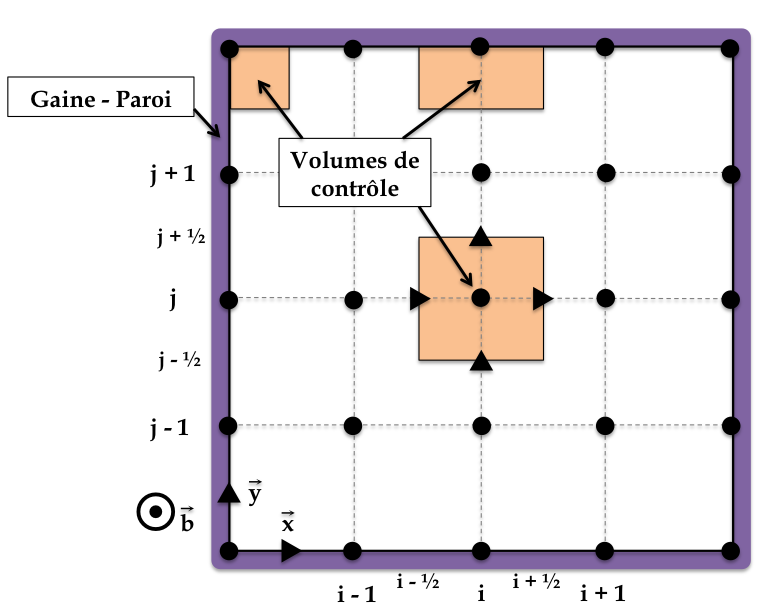
\includegraphics[height=64mm,width=80mm]{figures/grid.png}
{\caption{Maillage 2D pour les schémas volumes finis}
\label{maillage}}
\end{figure}

 \subsection{Fréquences}
 
 Une attention particulière est portée à description précise des 
 flux de matière et de chaleur fortement dépendants de la magnétisation du plasma. Une étape de prédiction est tenant compte de la force 


\subsection{Discrétisation temporelle}

\begin{equation}
S_s(T_e)=n^{k+1}n_gk_{s}^{iz}(T_e)
\end{equation}
où $n_g$ est la densité du gaz et $k_{s}^{iz}$ le coefficient d'ionisation spécifique à l'espèce.
\citep{Hemsworth}

\section{Vérification et validation}

\subsection{Etude de convergence en temps et en espace}
\subsubsection{Densité}
\subsubsection{Potentiel}
\subsubsection{Température}
\subsection{Influence du champ magnétique}
\subsection{Réponses à la température}

\bibliographystyle{alpha}
\bibliography{biblio}
